\documentclass{article}
\usepackage{blindtext}
\usepackage{amsmath}
\usepackage{multicol}
\usepackage{graphicx}
\usepackage[margin=1in]{geometry}
\begin{document}

Nathan Joshua B. Sucgang

\today

\begin{enumerate}
    \item[1.)] A router is used to cut locating notches on a printed circuit board. The vibration level at the surface of the board as it is cut is considered to be a major source of dimensional variation in the notches. Two factors are thought to influence vibration: bit size (A) and cutting speed (B). Two bit sizes ( 1/8and 1/16 in.) and two speeds (40 and 90 rpm) are selected, and four boards are cut at each set of conditions shown below. The response variable is vibration measured as the resultant vector of three accelerometers (x, y, and z) on each test circuit board.
    \begin{figure}[!htbp]
        \centerline{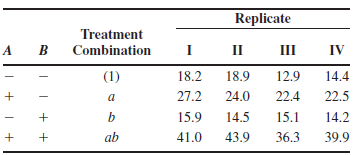
\includegraphics[width=10cm,height=8cm,keepaspectratio]{Picture 1.png}}
    \end{figure}  

    Find the sums of squares, degrees of freedom, mean squares, F test values, and F critical values. (20 pts)

    \begin{tabular}{|c|c|c|c|c|c|}
        \hline
        \textbf{Sources of Variation} & \textbf{Degree of Freedom} & \textbf{Sum of Squares} & \textbf{Mean Square} & \textbf{F-ratio} & \textbf{F-critical}\\
        \hline
        A & 1 & 8.31875 & 8.31875 & 0.05895 & 4.75 \\
        B & 1 & 3.80000 & 3.76875 & 0.02671 & 4.75 \\
        AB & 1 & 4.40000 & 4.35625 & 0.03087 & 4.75 \\
        Error & 12 & 1693.390625 & 141.1158854 & & \\
        Total & 15 & 1709.834375 & & & \\
        \hline
        \end{tabular}

        For A:

        Since $0.05895 < 4.75$, so fail to reject $H_0$.

        For B:

        Since $0.02671 < 4.75$, so fail to reject $H_0$.

        For AB: 

        Since $0.03087 < 4.75$, so fail to reject $H_0$.

    \newpage

    \item[2.)] The following represent the number of defects per 1000 feet in copper wire:
    
    1, 1, 3, 7, 8, 10, 5, 13, 0, 19, 24, 6, 9, 11, 15, 8, 3, 6, 7, 4, 9, 20, 11, 7, 18, 10, 6, 4, 0, 9, 7, 3, 1, 8, 12.
    \begin{enumerate}

        \item[a.)] What type of control chart should you use? Find the CL, the UCL, and the LCL. (5 pts)
        
        CL: 8.143, LCL: 3.175, UCL: 13.111

        \item[b.)] Plot the points on a control chart that includes the Western Electric pattern rules. (5 pts)
        
        \begin{figure}[!htbp]
            \centerline{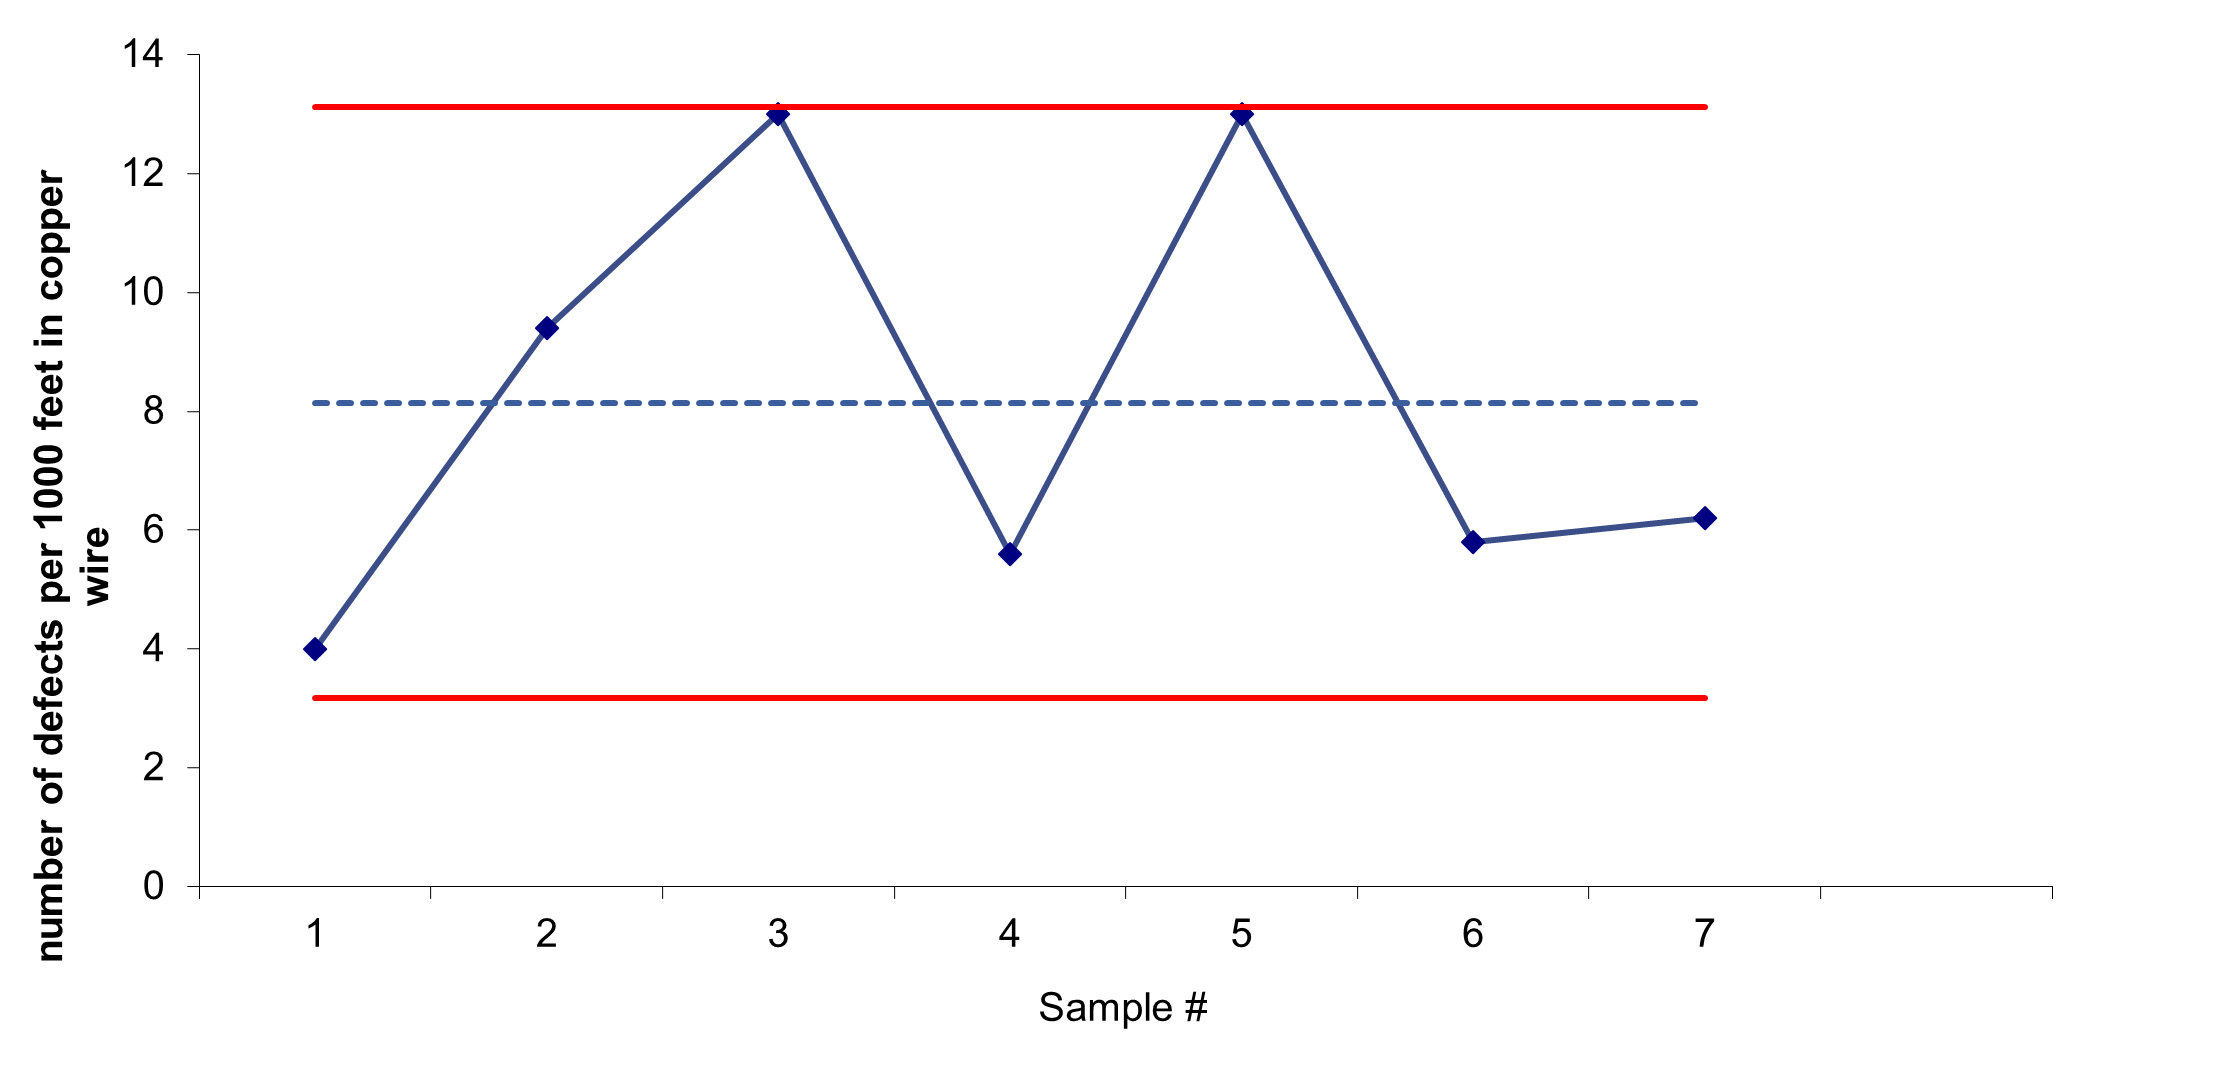
\includegraphics[width=10cm,height=8cm,keepaspectratio]{Picture 3.png}}
        \end{figure}

        \item[c.)] Do the data come from a controlled process? Why or why not. (5 pts)
        
        We can clearly see that all of the data does not exceed UCL and LCL. Therefore, the process mean is in statistical control. 

    \end{enumerate}

    \newpage
    
    \item[3.)] The following are the fractions defective of shaft and washer assemblies during the month of April in samples of n = 1500 each:
    \begin{figure}[!htbp]
        \centerline{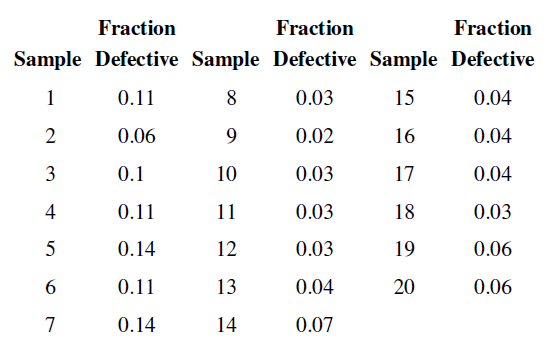
\includegraphics[width=10cm,height=8cm,keepaspectratio]{Picture 2.png}}
    \end{figure}
    \begin{enumerate}
        \item Set up a P chart for this process. Is this process in statistical control? (5 pts)
        
        $\bar{p}$: 0.000043, LCL: 2.9885405E-05, UCL: 5.6114595E-05
        \begin{figure}[!htbp]
            \centerline{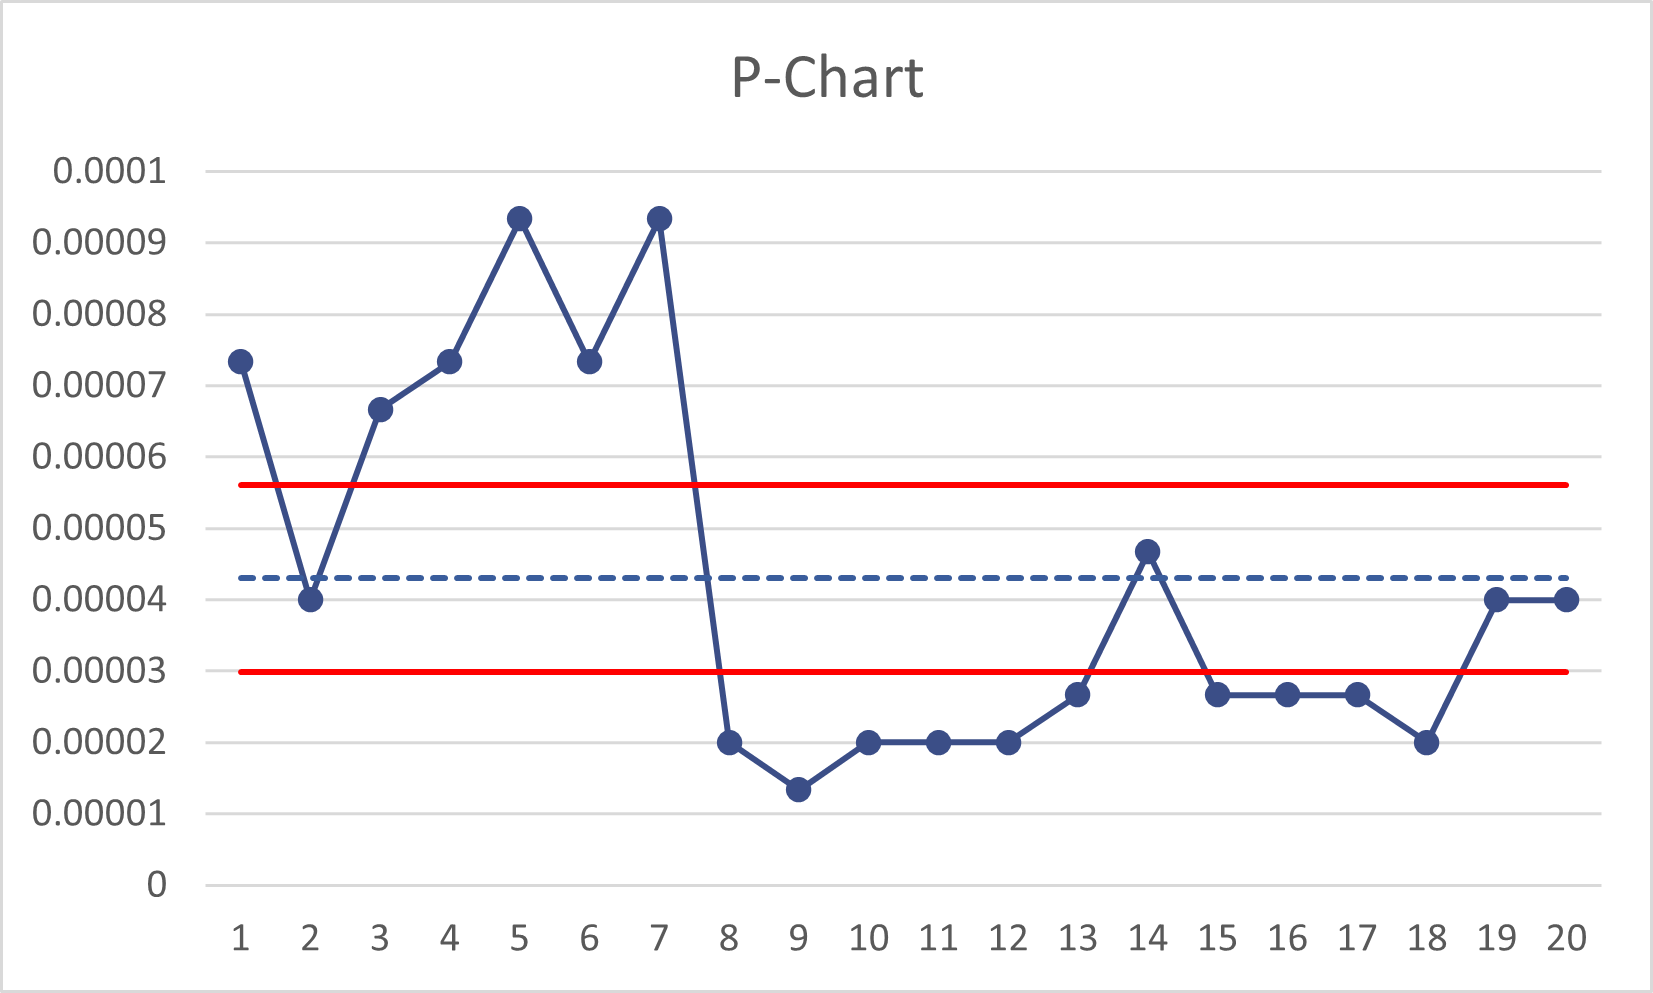
\includegraphics[width=10cm,height=8cm,keepaspectratio]{Picture 4.png}}
        \end{figure}

        We can see that the sample 1 - 7 is clearly above the upper control limit and We can also see that the sample 8 - 13, 15 - 18 is clearly below the lower control limit.
        Therefore, the process is not in statistical control. 

        \newpage

        \item Suppose that instead of n = 1500, n = 100. Use the data given to set up a P chart for this process. Revise the control limits if necessary. (5 pts)
        
        $\bar{p}$: 0.000645, LCL: -1.1665975E-04, UCL: 1.4066598E-03
        \begin{figure}[!htbp]
            \centerline{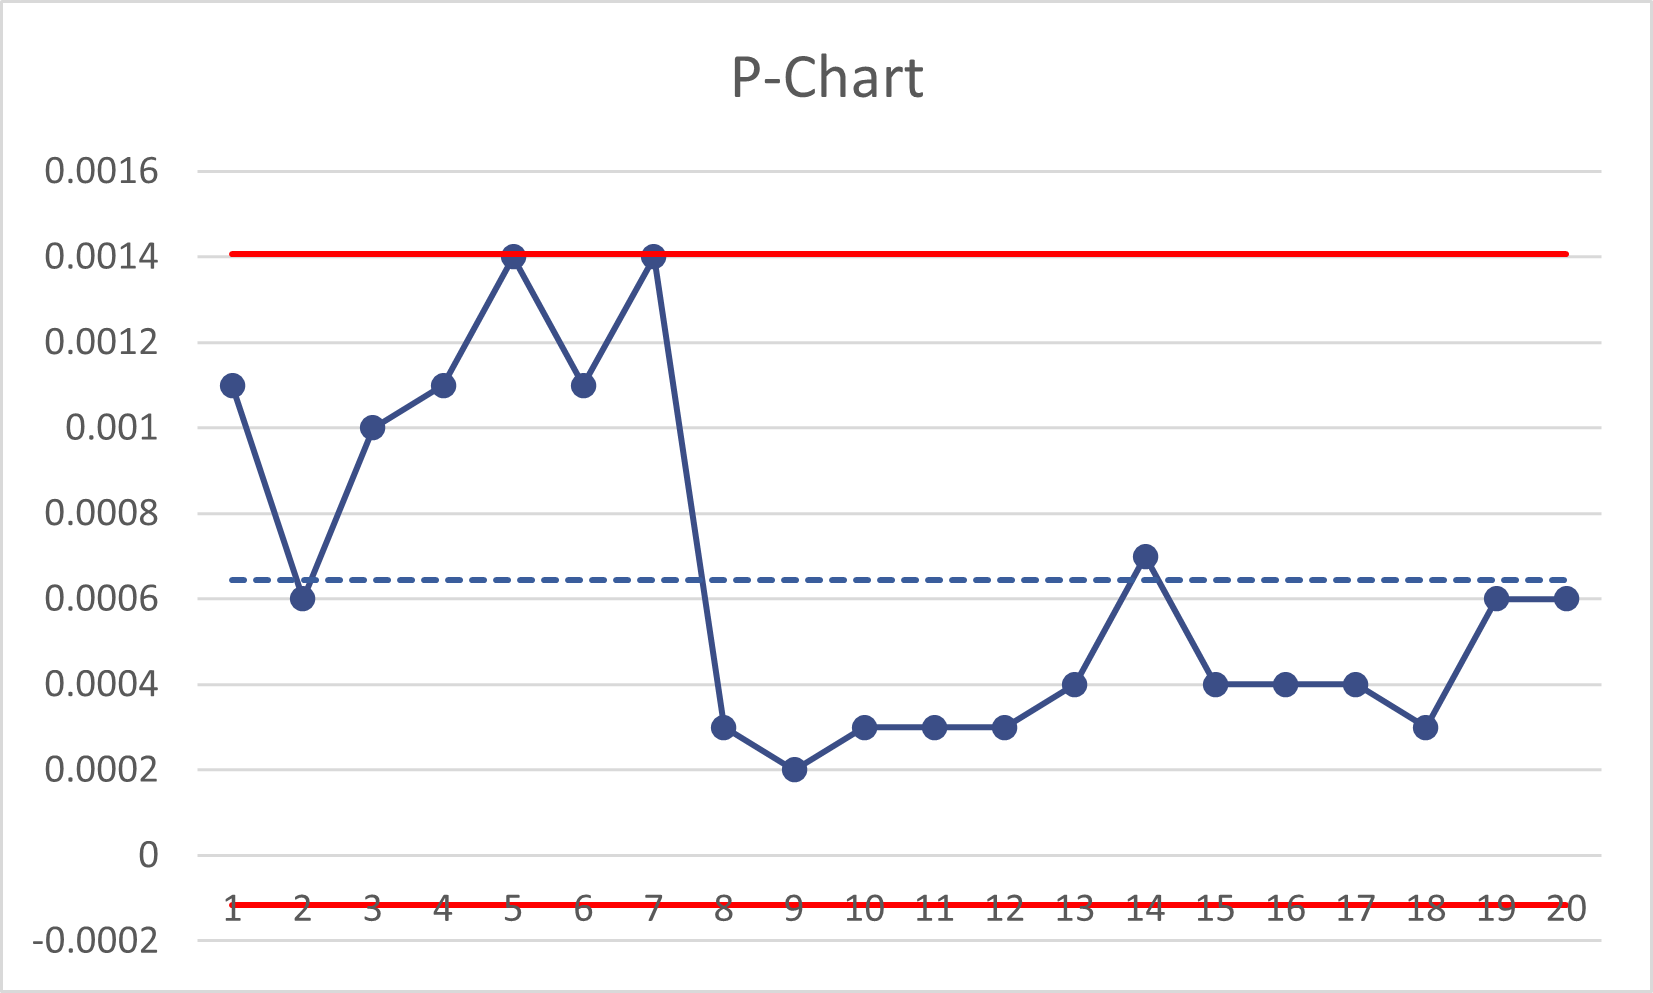
\includegraphics[width=10cm,height=8cm,keepaspectratio]{Picture 5.png}}
        \end{figure}

        We can clearly see that all of the data does not exceed UCL and LCL. Therefore, the process mean is in statistical control. 

        \item Compare your control limits for the P charts in parts (a) and (b). Explain why they differ. Also, explain why your assessment about statistical control differs for the two sizes of n. (5 pts)
        
        For n = 1500, we have $\bar{p}$: 0.000043. For n = 100, we have $\bar{p}$: 0.000645. They are different because the formula of $\bar{p} = \frac{\text{total number of defective}}{\text{total number of sample}}$, given that the number of defective does not change and only the total number of sample differ. 
        We can say that they have inverse relationship, if sample size is large then $\bar{p}$ is small and vice versa.  
        For smaller sample sizes (n), the variable-width approach may be more conservative, as it accounts for the increased uncertainty in the sample proportion. 
        Conversely, for larger sample sizes (n), the average sample size approach may be more effective, as it leverages the increased precision in the sample proportion.
    \end{enumerate}
\end{enumerate} 
\end{document}